% !TEX TS-program = xelatex
% !TEX encoding = UTF-8 Unicode
% !Mode:: "TeX:UTF-8"

\documentclass{resume}
\usepackage{zh_CN-Adobefonts_external} % Simplified Chinese Support using external fonts (./fonts/zh_CN-Adobe/)
% \usepackage{NotoSansSC_external}
% \usepackage{NotoSerifCJKsc_external}
% \usepackage{zh_CN-Adobefonts_internal} % Simplified Chinese Support using system fonts
\usepackage{linespacing_fix} % disable extra space before next section
\usepackage{cite}
\usepackage{multirow}

\begin{document}
\pagenumbering{gobble} % suppress displaying page number
% \begin{tabular}{cl}
%    \multirow{5}{1in}{
\includegraphics[width=0.88in]{avatar}} & \multirow{3}[]{}[]{}{宋彤雨} \\
%    & \phone{(+86) 180-8093-2513}\\
%    & \email{SDNanyflow@gmail.com}
% \end{tabular}
% Please add the following required packages to your document preamble:
% \usepackage{multirow}
\begin{table}[]
\begin{tabular}{ll}
\multirow{5}{1in}{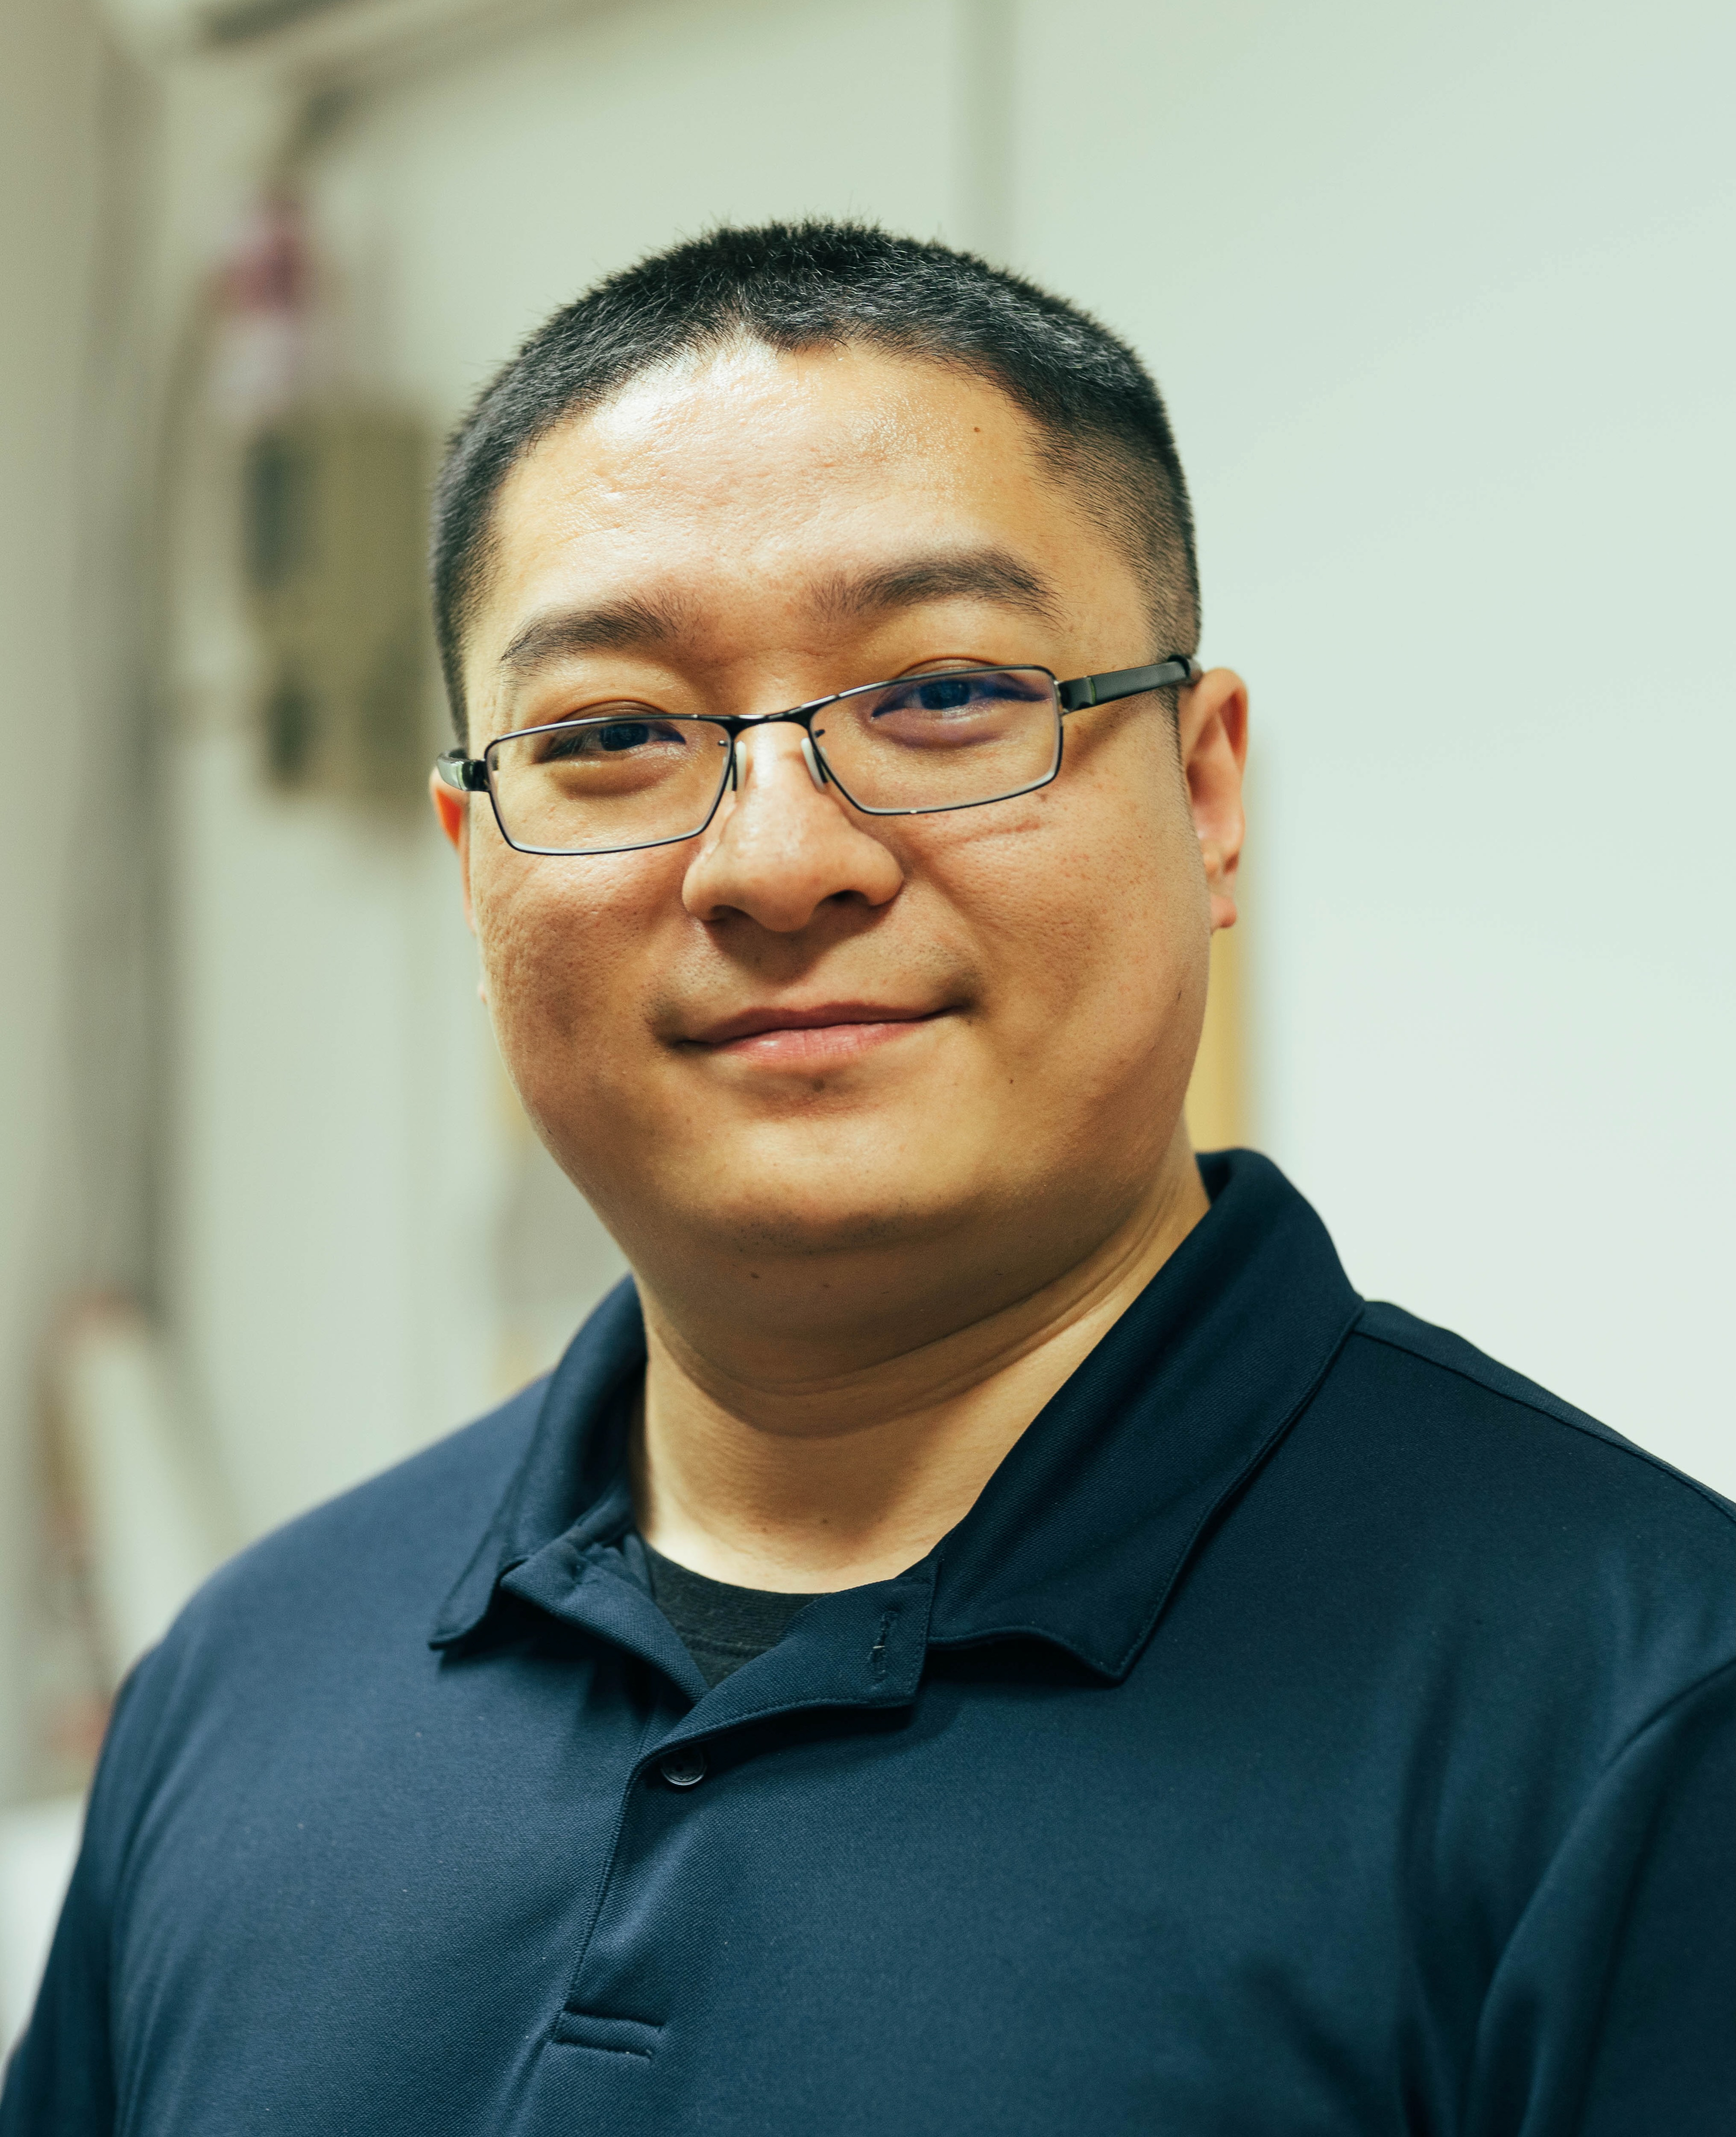
\includegraphics[width=0.88in]{sty}} & \multirow{4}{2in}{\LARGE{\textbf{\quad 宋彤雨}}} \\
                   &\\
                   &\\
                   & \phone{(+86) 180-8093-2513}\\
                   & \email{SDNanyflow@gmail.com}                 
\end{tabular}
\end{table}
% \name{你的大名}

% \basicInfo{
%   \email{yuanbin2014@gmail.com} \textperiodcentered\ 
%   \phone{(+86) 131-221-87xxx} \textperiodcentered\ 
%   \linkedin[billryan8]{https://www.linkedin.com/in/billryan8}}
 
\section{\faGraduationCap\  教育背景}
% \datedsubsection{\textbf{上海交通大学}, 上海}{2013 -- 至今}
% \textit{在读硕士研究生}\ 信息与通信工程, 预计 2016 年 3 月毕业
% \datedsubsection{\textbf{西安电子科技大学}, 西安, 陕西}{2009 -- 2013}
% \textit{学士}\ 通信工程
\datedsubsection{\textbf{电子科技大学},通信与信息系统,在读博士研究生(导师:王晟\; 教授)}{2014.9 - 2022.6}
\ 智慧网络与应用团队(李乐民院士团队),网络规划与优化实验室,光纤传输与通信教育部重点实验室
\datedsubsection{\textbf{电子科技大学},网络工程,工学学士}{2010.9 - 2014.6}
\ \textbf{排名5/102},国家奖学金,人民奖学金(3次)

\section{\faUniversity  学术成果}
\datedsubsection{\textbf{学术论文}}{}
\begin{enumerate}
  \item \textbf{Tongyu Song}, X. Tan, J. Ren, et al., DRAM: A DRL-based Resource Allocation Scheme for MAR in MEC.
  Digital Communications and Networks(DCN), 2022.(SCI期刊,中科院一区)
  % \\https://doi.org/10.1016/j.dcan.2022.04.014
  \item \textbf{Tongyu Song}, W. Hu, X. Tan, et al., FAST-RAM: a Fast AI-assistant Solution for Task Offloading and Resource Allocation in MEC. IEEE Global Communications Conference (GLOBECOM), 2020.(EI会议,CCF C类推荐会议)
  % \\http://ieeexplore.ieee.org/stamp/stamp.jsp?tp=\&arnumber=9322645\&isnumber=9321973
  \item \textbf{Tongyu Song}, W. Hu, X. Tan, et al., ARM: An Accelerator for Resource Allocation in Mobile Edge Computing. IEEE Global Communications Conference (GLOBECOM), 2019.(EI会议,CCF C类推荐会议)
  % \\http://ieeexplore.ieee.org/stamp/stamp.jsp?tp=\&arnumber=9014042\&isnumber=9013108
  \item \textbf{Tongyu Song}, W. Hu, W. Xu, et al., FAIR-AREA: A Fast AI-Based Joint Optimization of Rate Adaptation and Resource Allocation for DASH. IEEE Global Communications Conference (GLOBECOM), 2019.(EI会议,CCF C类推荐会议)
  % \\http://ieeexplore.ieee.org/stamp/stamp.jsp?tp=\&arnumber=9013477\&isnumber=9013108
  \item \textbf{Tongyu Song}, S. Wang, J. Ren, et al., JRA2: Joint Optimization of Resource Allocation and Rate Adaptation for DASH Services. IEEE International Conference on Communications (ICC), 2018.(EI会议,CCF C类推荐会议)
  % \\http://ieeexplore.ieee.org/stamp/stamp.jsp?tp=\&arnumber=8422841\&isnumber=8422068
  \item \textbf{Tongyu Song}, X. Tan, J. Ren, et al., COLLAR: Adaptation Scheme for Mobile Augmented Reality in Mobile Edge Computing. Future Generation Computer Systems.(SCI期刊,中科院一区,评审中)
  \item\textbf{Tongyu Song}, X. Guo, J. Ren, et al., CO-CAST: Scheme for routing and bandwidth allocation for multiple consortium blockchain based on deep reinforcement learning. Future Generation Computer Systems.(SCI期刊,中科院一区,评审中)
  \item\textbf{Tongyu Song}, J. Zheng, J. Ren, et al., CO-NEXT: Scheme for intelligent topology optimization for ad-hoc network based on multi-agent DRL. IEEE Internet of Things Journal.(SCI期刊,中科院一区,评审中)
\end{enumerate}
\datedsubsection{\textbf{发明专利}}{}
\begin{enumerate}
    \item 一种多联盟链共识算法的网络时延优化方法, CN202110591340.6.(第一发明人)
    \item 基于深度学习的智能视频码率调整及带宽分配方法, CN202110097764.7.(第一发明人)
    \item 基于智能体深度增强学习的多边缘基站联合缓存替换方法, CN202110599821.1.(第一发明人)
    \item 基于多智能体增强学习的WSN能量效率优化路由方法, CN202210378218.5.(第二发明人,审批中)
\end{enumerate}
\datedsubsection{\textbf{参与的国际标准工作}}{}
\begin{enumerate}
    \item ITU-T H.643.1 Architecture for deployment of information centric network(支持信息中心网络的部署的架构),2019年8月正式发布执行
    \item ITU-T F.746.5 Requirements for deployment of information centric network(信息中心网络的部署的要求),2017年3月正式发布执行
    \item ITU-T F.746.6 Requirements for a name resolution service in information-centric networks(信息中心网络中名字解析服务的要求),2017年12月正式发布执行
\end{enumerate}
\datedsubsection{\textbf{学术专著}}{}
《AI技术应用:网络资源管理》,人民邮电出版社(第一作者,撰写中,2022.10出版)
\section{\faCogs 研究方向及研究实例}
\datedsubsection{\textbf{利用深度学习快速求解复杂优化问题}}{}
\begin{enumerate}
  \item \textbf{多DASH视频流码率选择和带宽资源分配联合优化}
  \\ 高质量的DASH视频流服务需要客户端和网络资源管理策略的协同,但是多视频流码率选择和带宽资源联合分配本身是困难的。这种困难体现为联合优化问题求解难度大,实际部署中对算法执行速度要求高。采用深度学习和监督学习框架,首先基于广义benders分解产生问题实例和对应最优解的样本数据集(JRA2算法,对应论文5),然后设计了适配问题结构的DNN从而实现快速求解(FAIR-AREA方案,对应论文2)。
  \item \textbf{移动边缘计算(MEC)中任务卸载和计算资源分配联合优化}
  \\ MEC场景中 处理的多为时延敏感业务,因而对资源管控机制的处理速度有较高要求。用户任务的卸载策略和计算资源的分配是MEC中的关键问题,但目前缺乏快速求解方面的工作。采用深度学习和监督学习框架,设计了快速求解方案(ARM方案,对应论文3),针对DNN特性对原始优化问题进行拆分,将用户任务卸载转化为多分类问题。在MEC服务器具有单一任务类型约束的情况下,设计了快速求解方案(FAST-RAM方案,对应论文2)。方案中设计了两个级联的DNN分别决策服务器应处理的任务类型和具体任务的卸载策略。在特征空间设计时,考虑方案的可扩展性,设计了用户任务的特征提取方案。
\end{enumerate}
\datedsubsection{\textbf{基于深度增强学习的动态资源管控}}{}
\begin{enumerate}
  \item \textbf{移动增强现实业务(MAR)中服务器参数动态配置和计算资源分配}
  \\ 因为MAR客户端具有自适应调整图片处理请求生成频率和图片大小的能力,精细的网络资源管控需要设计动态服务器参数配置和为每个客户端 分配资源的机制。设计了两个方案,方案一使用DDPG(DRAM方案,对应论文1),针对业务特征设计了反应用户请求紧迫性的状态空间和符合资源分配机制的动作空间;方案二使用MADDPG(论文撰写中)将DRAM方案拆分为两个级联的虚拟智能体,分别决策服务器配置和用户资源分配方案。多智能体方案相对单智能体方案能够提升10\%的性能,但是收敛过程更长。
  \item \textbf{MAR和DASH业务中多客户端应用层参数协同动态调整策略} 
  \\ 在多个采用自适应策略的客户端竞争资源时,不加协作的各自独立决策在资源使用角度是低效的。本实例中采用COMA在MAR(COLLAR方案,对应论文6)和DASH(论文撰写中,对应专利2)业务中设计了客户端协同动态调整策略。两个方案都针对各自的业务特点设计了奖励函数设计,同时都与单智能体算法进行了对比,验证了设计多智能体方案的必要性。
  \item \textbf{MEC中多基站联合缓存替换策略} 
  \\ 边缘缓存资源总量小同时需要面对用户需求内容流行度的动态变化,现有研究缺乏边缘基站之间的协同机制,所以本实例设计了基于COMA的多基站联合缓存替换策略(对应专利3)。设计了及时反映内容流行度的状态空间设计,同时针对业务特点设计了动作空间和奖励函数。
  \item  \textbf{基于BaaS的多联盟链路由动态规划和带宽分配}
  \\ 现有研究缺乏联盟链网络层性能优化的工作,同时由于多联盟链区块广播中的路由规划是经典的多多播树路径规划问题,结合带宽资源的分配,问题本身也是困难和少有研究的。本实例中使用MADDPG为各联盟链设计了路由动态调整方案(CO-CAST方案,对应论文7,专利1),针对区块链中区块的验证过程设计了状态空间和最大化上层交易吞吐的带宽分配算法。
  \item \textbf{无线传感网动态拓扑规划}
  \\ 现有的针对能量效率的WSN拓扑规划工作多基于固定算法,现有表现良好的算法实现难度大。近期出现的利用DRL的方法在算法范型上难以保证模型的正确性。本实例设计了基于平均场多智能体DRL算法的动态路由规划方案(CO-NEXT方案,对应论文8,专利4),利用平均场理论简化训练过程,同时在动作空间设计中考虑提高从智能体动作到实际路由方案的映射的有效性和可行性。
\end{enumerate}
\section{\faUsers 科研项目}
\datedsubsection{1. \textbf{资源动态适配机制与理论}}{}
国家重点基础研究发展计划(973计划),2013CB329103,373万元,2013/01/01-2017/08/31

\faChevronRight 对应DASH业务研究实例

\datedsubsection{2. \textbf{软件定义网络中应用与网络合作的资源分配模型及机制研究}}{}
国家自然科学基金,面上项目,6167011865,80.5440万元,2017/01/01-2020/12/31

\faChevronRight 对应DASH和MEC中的研究实例。
\datedsubsection{3. \textbf{随愿共享的业务能力协同互联技术}}{}
国家重点研发计划,2020YFB1807804,540万元,2020/12/01-2023/11/30

\faChevronRight 对应MEC中多基站协同缓存的研究实例

% \datedsubsection{国家重点研发计划,2020YFB1807805,按需服务的智联网管控原型系统研制}{73.5万元,2020/12/01-2023/11/30}

\datedsubsection{4. \textbf{差异化服务智能适配与路由}}{}
国家重点研发计划,2019YFB1802802,162万元,2020/01/01-2022/12/31

\faChevronRight 对应联盟链业务的研究实例

% 国家自然科学基金,面上项目,62072079,面向下一代网络的可编程测量架构及关键测量方法,58万元国家
\datedsubsection{5. \textbf{类生物免疫机制的网络安全防护理论与方法}}{}
自然科学基金联合基金项目,U20A20156,269万元,2021/01/01-2024/12/31

\faChevronRight 负责设计横向移动场景中的智能攻击和防御策略、设计对现有攻击者策略进行模仿学习的智能体
\\以及智能攻防策略的可解释性工作

\datedsubsection{6. \textbf{基于多智能体协同学习的网络资源管控机制研究}}{}
国家自然科学基金青年基金,62001087,24万元,2021/01/01-2023/12/31

\faChevronRight 对应使用多智能体DRL方法的研究实例
\datedsubsection{7. \textbf{网络流量智能规划技术}}{}
中央军委装备发展部,“十三五”全军公用信息系统装备预先研究项目,JZX6Y202001010034,226万,2020/01-2021/06

\faChevronRight 利用SDN交换机搭建了DASH业务测试平台,并测试了多客户端协同动态调整策略的性能 

% \section{\faUsers\ 实习/项目经历}
% \datedsubsection{\textbf{黑科技公司} 上海}{2015年3月 -- 2015年5月}
% \role{实习}{经理: 高富帅}
% xxx后端开发
% \begin{itemize}
%   \item 实现了 xxx 特性
%   \item 后台资源占用率减少8\%
%   \item xxx
% \end{itemize}

% \datedsubsection{\textbf{分布式科学上网姿势}}{2014年6月 -- 至今}
% \role{Golang, Linux}{个人项目,和富帅糕合作开发}
% \begin{onehalfspacing}
% 分布式负载均衡科学上网姿势, https://github.com/cyfdecyf/cow
% \begin{itemize}
%   \item 修复了连接未正常关闭导致文件描述符耗尽的 bug
%   \item 使用Chord 哈希 URL, 实现稳定可靠地分流
%   \item xxx (尽量使用量化的客观结果)
% \end{itemize}
% \end{onehalfspacing}

% \datedsubsection{\textbf{\LaTeX\ 简历模板}}{2015 年5月 -- 至今}
% \role{\LaTeX, Python}{个人项目}
% \begin{onehalfspacing}
% 优雅的 \LaTeX\ 简历模板, https://github.com/billryan/resume
% \begin{itemize}
%   \item 容易定制和扩展
%   \item 完善的 Unicode 字体支持,使用 \XeLaTeX\ 编译
%   \item 支持 FontAwesome 4.5.0
% \end{itemize}
% \end{onehalfspacing}

% % Reference Test
% %\datedsubsection{\textbf{Paper Title\cite{zaharia2012resilient}}}{May. 2015}
% %An xxx optimized for xxx\cite{verma2015large}
% %\begin{itemize}
% %  \item main contribution
% %\end{itemize}

% \section{\faCogs\ IT 技能}
% % increase linespacing [parsep=0.5ex]
% \begin{itemize}[parsep=0.5ex]
%   \item 编程语言: C == Python > C++ > Java
%   \item 平台: Linux
%   \item 开发: xxx
% \end{itemize}

% \section{\faHeartO\ 获奖情况}
% \datedline{\textit{第一名}, xxx 比赛}{2013 年6 月}
% \datedline{其他奖项}{2015}

% \section{\faInfo\ 其他}
% % increase linespacing [parsep=0.5ex]
% \begin{itemize}[parsep=0.5ex]
%   \item 技术博客: http://blog.yours.me
%   \item GitHub: https://github.com/username
%   \item 语言: 英语 - 熟练(TOEFL xxx)
% \end{itemize}

% %% Reference
% %\newpage
% %\bibliographystyle{IEEETran}
% %\bibliography{mycite}
\section{\faThumbsOUp 竞赛获奖}
% increase linespacing [parsep=0.5ex]
\begin{itemize}[parsep=0.2ex]
  \item 第一届全国高校软件定义网络(SDN)应用创新开发大赛\textbf{全国一等奖}\; 2014.8
  \\\faChevronRight 尽力而为网络中在线视频QoS保障解决方案\\ \textit{https://www2.scut.edu.cn/sdn2014/2014/0904/c4242a75928/page.htm}
\end{itemize}
\section{\faComments 其它实践}
% increase linespacing [parsep=0.5ex]
\begin{itemize}[parsep=0.2ex]
    \item 组建团队首个人工智能网络资源管控小组,累计指导3名硕士研究生和14名本科生毕业设计
\end{itemize}
\end{document}
